% Makes TeXShop able to find master LaTeX file to compile
% !TeX root = ../main.tex

% Get the width ot the longest/largest title. This will be the main title.
\settowidth{\unitlength}{\titleMain}

\begin{titlingpage}
\centering

% Print the upper brace.
{
	\color{LightGoldenrod}
	\resizebox*{\unitlength}{\baselineskip}{\rotateright{$\}$}}
} \\ [\baselineskip]

% Print the main title.
{
	\color{Sienna}
	\titleMain
} \\ [\baselineskip]

% Print the subtitle.
%{
%	\color{RosyBrown}
%	\titleSub
%} \\ [\baselineskip]

% Print the pre-title.
{
	\color{RosyBrown}
	\titleSemester \\
	%\titleDocument\\
}

% Print the lower brace.
{
	\color{LightGoldenrod}
	\resizebox*{\unitlength}{\baselineskip}{\rotateleft{$\}$}}
}

% Fill blank space.
\vfill

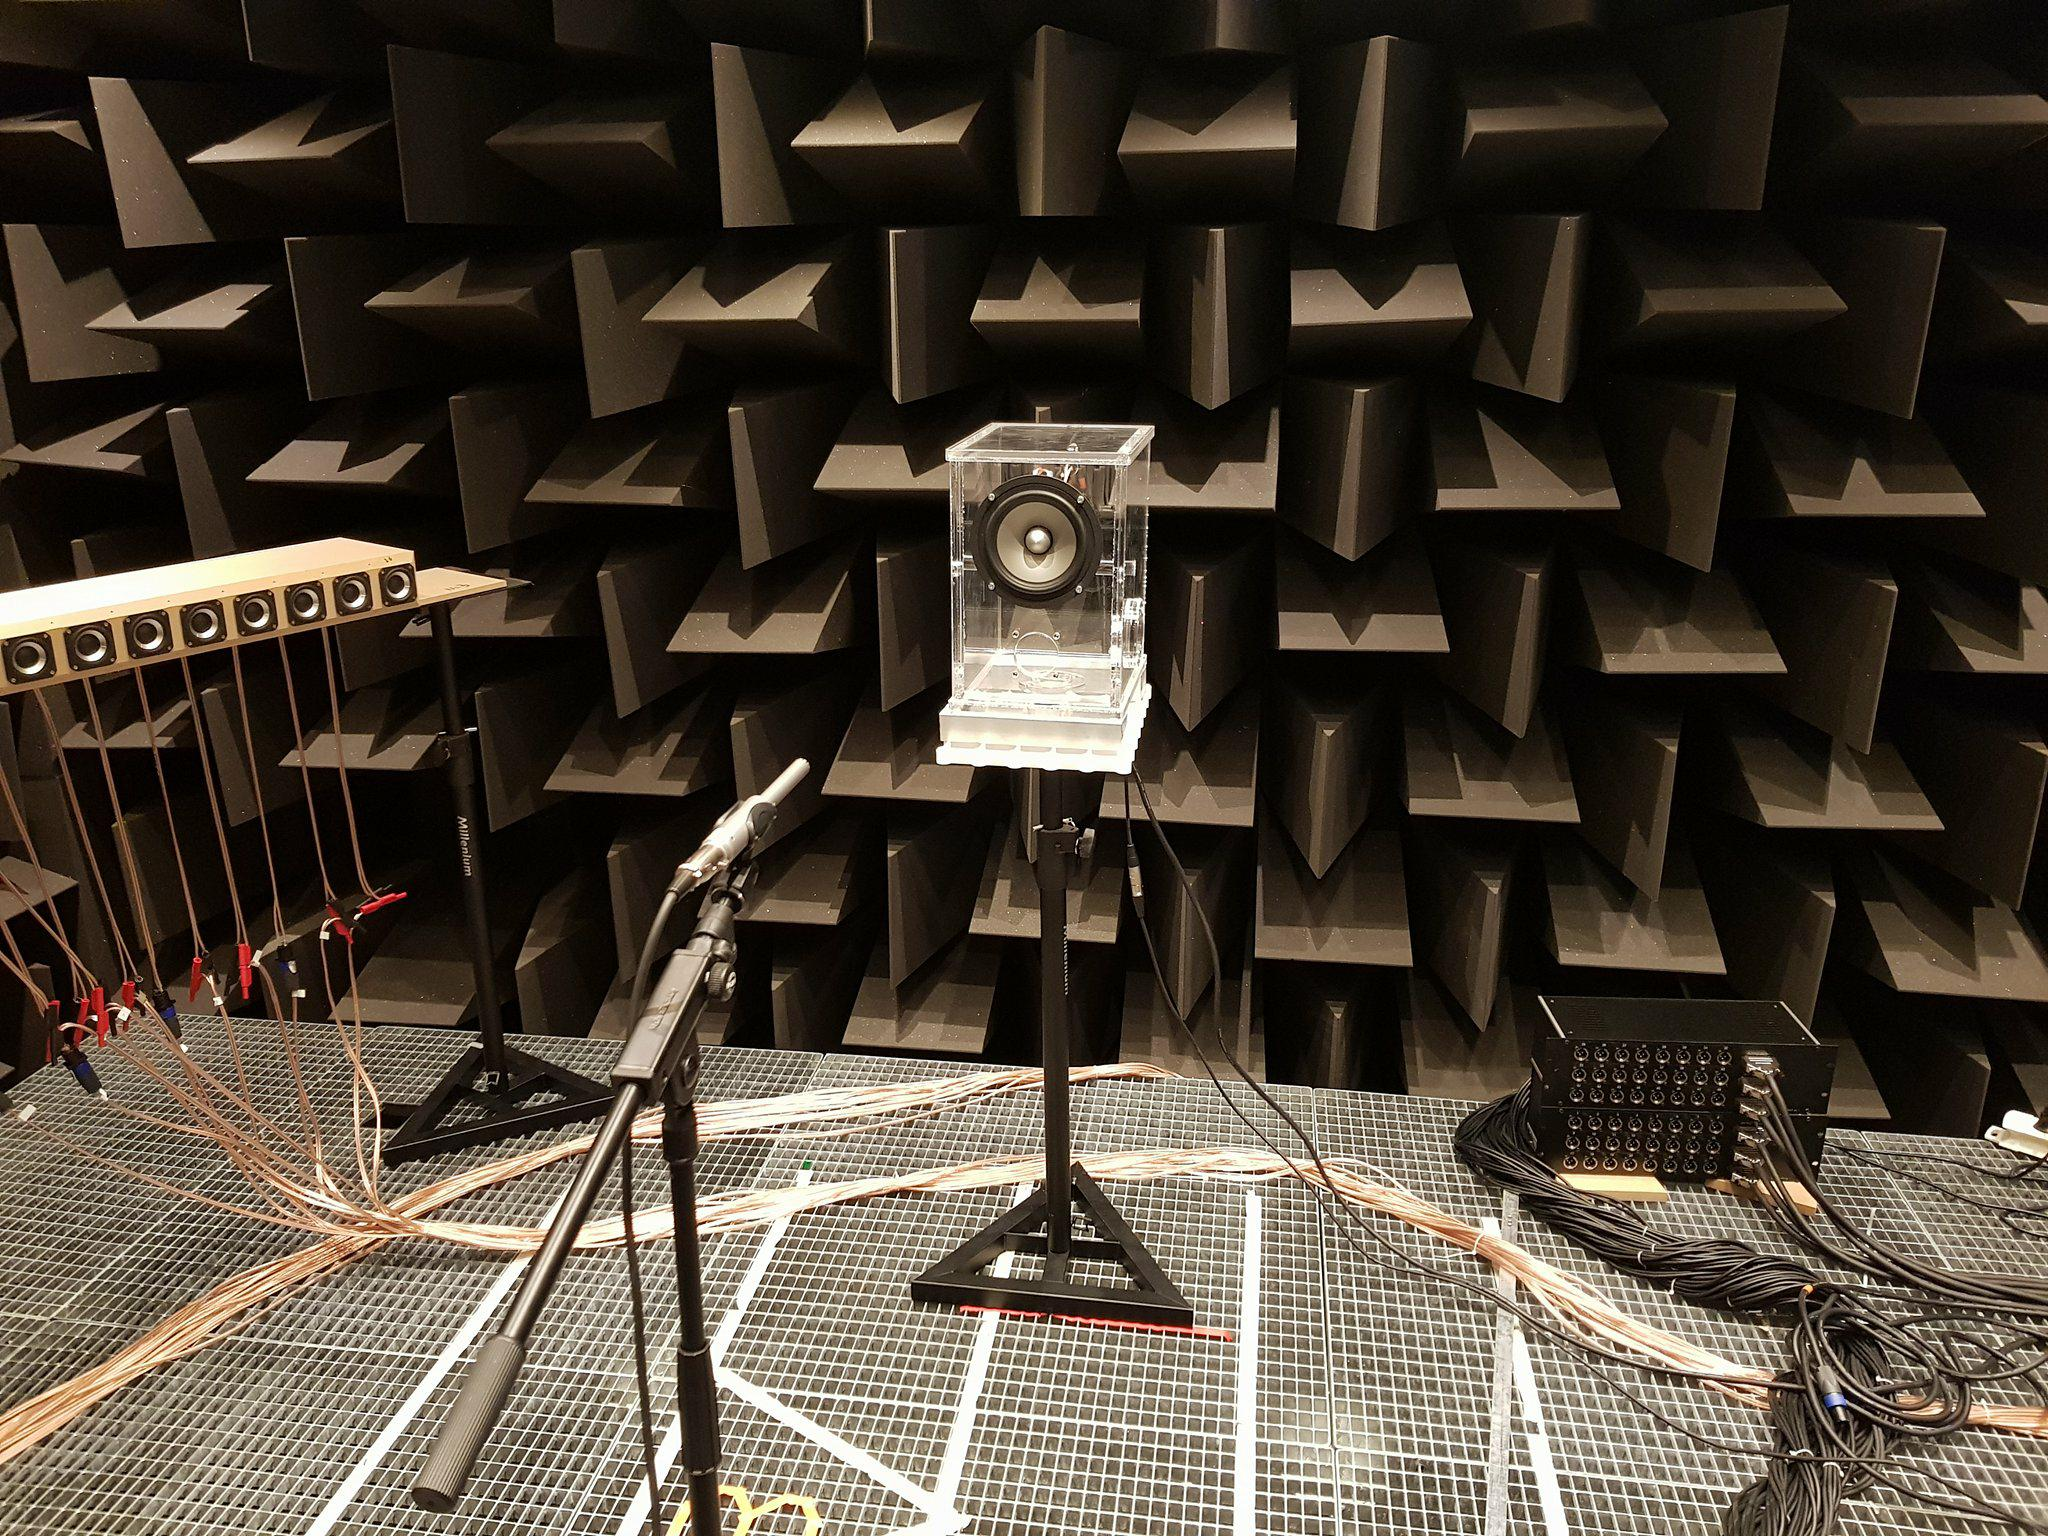
\includegraphics[width=12cm]{gfx/meas_setup.jpg}

% Fill blank space.
\vfill

% Print group members.
\begin{tabu} to \linewidth {X[1,c] X[1,c]}
\authorOneName						& \authorTwoName \\
\authorOneID						& \authorTwoID \\
									& \\
\end{tabu} \\ [2\baselineskip]

% Print advisor.
{
	{\Large Advisor} \\
	\advisorName
}

\end{titlingpage}
